\section{Property Prover Architecture\levi{remove this section?}}
\label{sec:architecture}

In this section we detail the operational artifacts used to implement the
algorithms described the previous sections. These artifacts are fully derived
from the source and target metamodels the DSLTrans transformation under
verification, and can be seen as a `compilation' step that need to be built for
each DSLTrans transformation in order to verify it. These artifacts can be
automatically built using higher-order transformations (HOTs), although for the
time being we have executed these HOTs as a manual step. We provide this section
in order to prove that the implementation of our verification technique follows
MDE principles: all artifacts are explicitly modelled by the appropriate
metamodels, and computations are performed using model transformations.

Figure~\ref{fig:verif_tool_arch} shows the higher order transformations needed
by our framework, along with other required artifacts such as metamodels and
models. Describing text will follow with a brief description of each HOT.

\begin{figure}[h!] \centering 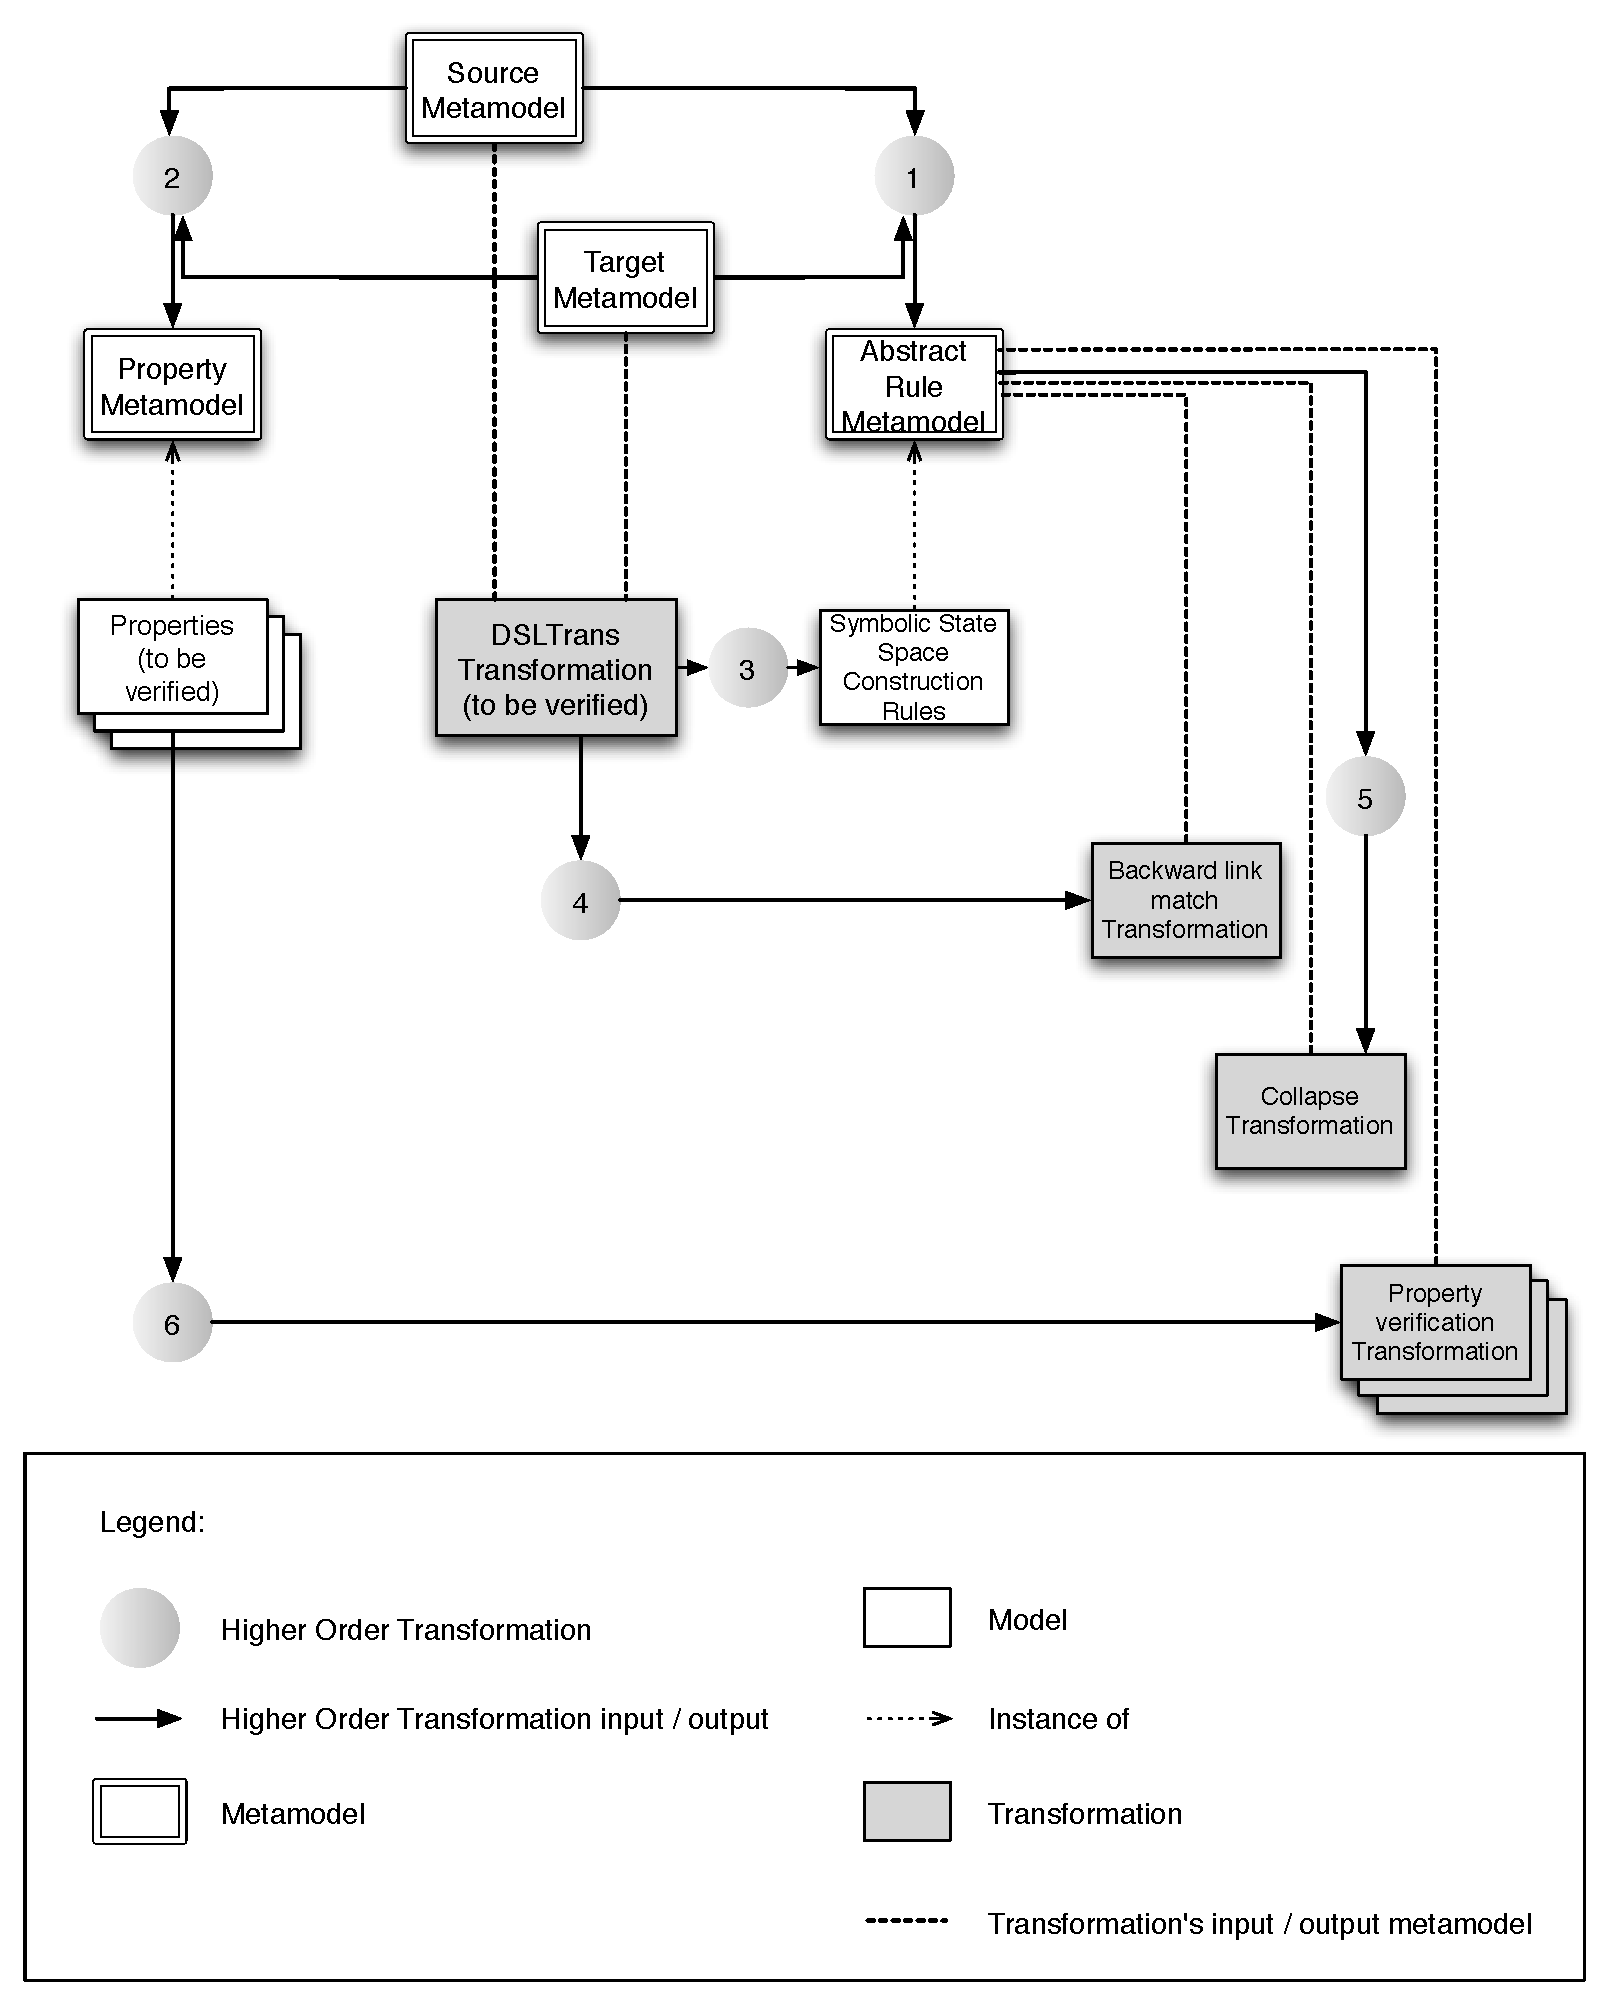
\includegraphics[scale=.45]{./figures/dsltrans_verification_architecture.pdf}
	\caption{Verification Tool Architecture}
	\label{fig:verif_tool_arch}
\end{figure}

\begin{enumerate}

  \item\label{label:abstract_rule_metamodel_hot} \textbf{Generate the
  \emph{abstract rule metamodel}}: this HOT takes as input the source and target
  metamodels of the transformation being analysed, and returns a metamodel in
  which an abstract form of the transformation rules can be written. Such a
  metamodel for the police station transformation can be observed in
  figure~\ref{fig:abstract_rule_metamodel_station_trafo}. The purpose of these
  abstract rules is to be the basic building blocks during symbolic execution
  construction.\\

  \item \textbf{Generate the \emph{property metamodel}}: this HOT also takes the
  source and target metamodels of the transformation. What is produced is the
  metamodel which will be used to express properties about the transformation.
  For example, the properties in  figures~\ref{fig:dsltrans_prop1}
  and~\ref{fig:dsltrans_prop2} are written using the \emph{property metamodel}
  generated for the Police Station transformation.\\

  \item \textbf{Generate the \emph{symbolic execution construction rules}}: this
  HOT builds a set that models that represent the transformation's rules, using
  the \emph{abstract rule metamodel}. These rules are then manipulated during
  path condition construction. As an example, the rules in the path
  conditions in the state space construction section
  (figures~\ref{fig:non_mergeable_symb_states},~\ref{fig:mergeable_symb_states}
  and~\ref{fig:mergeable_symb_states_repetition}) are \emph{symbolic execution
  construction rules}.\\

  \item \textbf{Generate the \emph{backward link match transformation}}: builds
  the query transformation responsible for checking whether a graph including
  backward links exists in a path condition. This is used in state space
  creation, where the existence of backward links between rule elements must be
  queried. The input metamodel of the backward link match transformation is the
  \emph{abstract rule metamodel}.\\

  \item \textbf{Generate the \emph{rule combination to path condition
  transformation}}: this HOT takes as input the \emph{abstract rule metamodel}
  generated in step~\ref{label:abstract_rule_metamodel_hot} and generates the
  transformation which transforms rules combinations into path conditions (which
  are both instances of the \emph{abstract rule metamodel}). This transformation
  has the \emph{abstract rule metamodel} as both source and target metamodel.\\

  \item \textbf{Generate the \emph{property verification transformation}}: this
  HOT generates three query transformations for each transformation property to
  be verified:
  \begin{itemize}
    \item a query transformation that checks whether the individual model
    elements present in the property are present in a path condition
    \item a second query transformation that checks whether the match part of the
    property is a subgraph of the match part of a path condition
    \item a third query transformation that checks whether the whole property is a subgraph of
    a path condition.
  \end{itemize}
  
  All query transformations have as source metamodel the \emph{abstract rule
  metamodel}. These transformations are then used in
  section~\ref{sec:verif_dsltrans_props}.
\end{enumerate}

\begin{figure}[h!] \centering 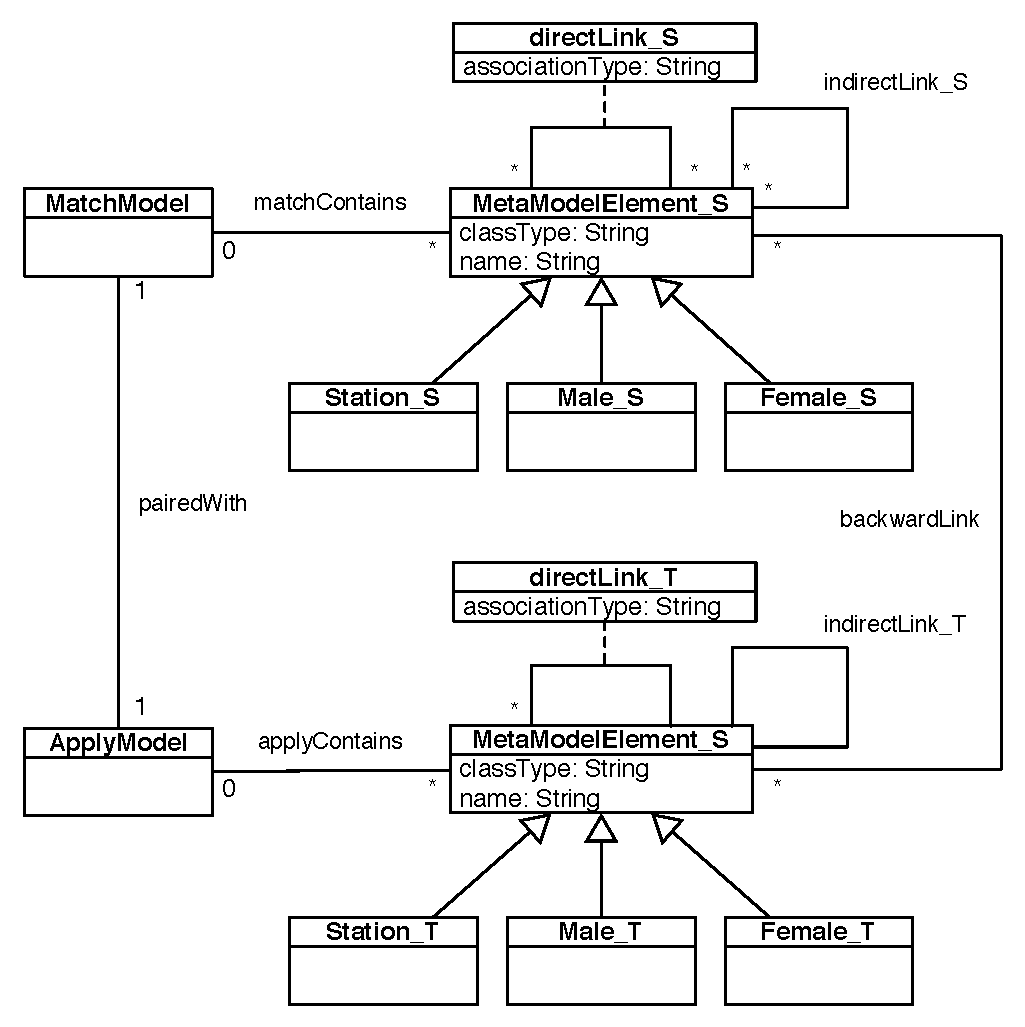
\includegraphics[scale=.6]{./figures/abstract_rule_metamodel.pdf}
	\caption{Abstract Rule Metamodel for the Police Station Transformation}
	\label{fig:abstract_rule_metamodel_station_trafo}
\end{figure}


% \begin{figure}[h!] \centering 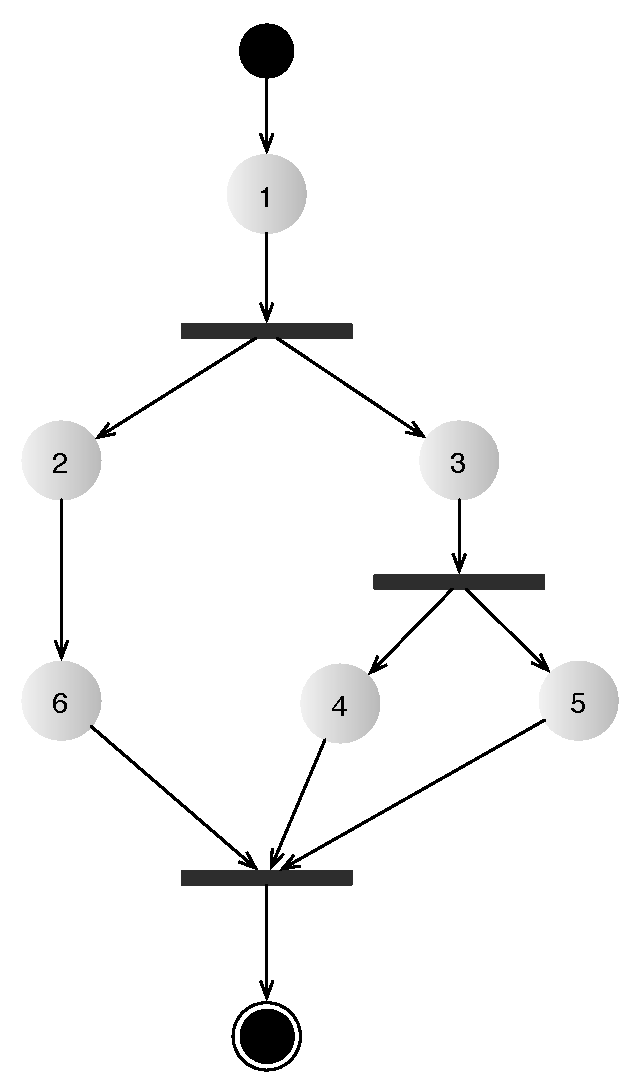
\includegraphics[scale=.45]{./figures/hot_activity_diagram.pdf}
% 	\caption{Activity Diagram Repesentation of the HOTs Composing the Verification Tool Architecture}
% 	\label{fig:activity_diagram_verif_tool_arch}
% \end{figure}

